\section{Introduction}
\label{sec:intro}

\begin{figure}[t]
  \centering
  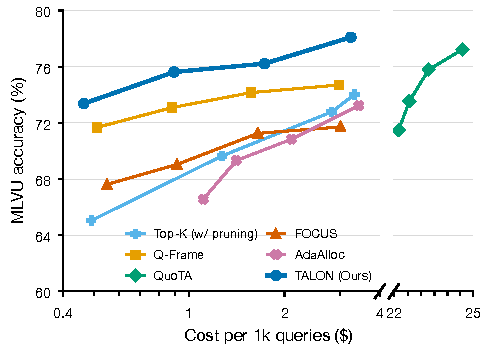
\includegraphics[width=\linewidth]{fig/budget_curve.pdf}
  \caption{\TODO{}}
  \label{fig:budget}
\end{figure}

\fyy{It turns out token compression is a popular method for video understanding (e.g., \href{https://arxiv.org/pdf/2510.07915}{retrieve-then-compress} and \href{https://arxiv.org/abs/2410.17434}{adaptive compression}). See my Teams message.}

\fyy{Therefore, a safer and better title and narrative should be
something like ``Efficient Video RAG through Token Allocation''.
Our keywords are token efficiency and token allocation (in a globally optimal manner, rather than greedy, independent compression).}

\fyy{My current thinking for the intro outline is as follows
(each point is a paragraph):
\begin{enumerate}
\item \textit{Problem \& importance.}
Briefly introduce VLM-based video understanding, then quickly
move to our problem setting of \textit{long} video understanding.
Establish its importance through concrete application domains.
\item \textit{RAG is commonly used for long video understanding.}
Processing all tokens from long videos can easily
exceed VLM context windows and incur high compute costs.
Therefore, existing systems widely resort to
RAG, notably embedding-based and graph-based approaches,
to supply relevant
visual or textual evidence for each query.
\item \textit{Limitations of existing approaches.}
Graph-based RAG achieves high benchmark accuracy,
but video ingestion is expensive and often wasted
since users tend to ask questions sporadically.
Embedding-based RAG is more lightweight, but our motivating
experiments in Section 2 reveal its limitations.
Adding tokens to a relevant frame yields diminishing returns.
Although video token compression mitigates this issue,
independently compressing retrieved frames
is also suboptimal,
as a different allocation of the global token budget
could reveal useful evidence in other frames.
\item \textit{Our insight and method.}
These limitations motivate us to jointly allocate
tokens across frames according to their contribution
to answering the query.
We present \name, a token-efficient video RAG framework
that preserves QA accuracy.
\name formulates video RAG as a token allocation problem
under a limited budget.
\item \textit{Challenges faced by \name and our solutions.}
Challenge 1 / solution 1 centers on
offline profiling of token value
and exact token allocation.
Challenge 2 / solution 2 is multi-turn conversations.
\item \textit{Evaluation highlights.}
\item \textit{Contributions and three bullet points.}
\end{enumerate}
}

paragraph 1: introduce video understanding

paragraph 2: highlight the problem of long context video understanding, introduce RAG methods for video understanding

paragraph 3: prior work is frame level, admits every frame at equal cost, however, relevant frames vary in relevance point to Fig X (x axis: frames, y axis relevance score). motivate token level design.

paragraph 4: highlight unique challenges,  characteristics we want from a strong design. 

paragraph 5: We introduce a plug-and-play \textbf{T}oken \textbf{AL}locati\textbf{ON} (\name) framework. quick pass through the framework, should demonstrate points in paragraph 4 are addressed.

% Our contributions are as follows:
% \begin{itemize}
%   \item We introduce \name, a plug-and-play framework that moves existing VideoRAG systems from frame-level RAG to token-level RAG.
%   \item We design a low-cost token scheduling algorithm from a principled optimization perspective, which jointly allocates tokens across frames and transcripts, using each modality for what it does best, and composes the resulting evidence into a temporally ordered storyboard. It improves on prior keyframe selection and token allocation methods both theoretically and empirically.
%   \item We extend token scheduling to multi-turn conversations, where the attention of the VLM updates the allocation of frames it has already seen, and new tokens are appended to the KV cache so that the total prefill stays bounded however long the conversation lasts.
%\end{itemize}
Across multiple VideoRAG backbones, \name achieves \todo{[TODO: A--B]}$\times$ higher accuracy than conventional frame retrieval and prior keyframe selection methods at matched compute budgets.


